\documentclass[14pt]{extarticle}
% \documentclass[14pt]{article}

% \usepackage[style=authoryear,maxbibnames=9,maxcitenames=2,uniquelist=false,backend=biber,doi=false,url=false]{biblatex}
% \addbibresource{$BIB} % bibtex location
% \renewcommand*{\nameyeardelim}{\addcomma\space} % have comma in parencite
\usepackage{natbib}

\usepackage{xcolor}
\usepackage{amsmath}
\newcommand{\tuple}[1]{ \langle #1 \rangle }
%\usepackage{automata}
\usepackage{times}
\usepackage{ltablex}
\usepackage{tasks}

%%%%%% Template
\usepackage{hyperref}
\hypersetup{colorlinks=true,allcolors=blue}

\usepackage{vmargin}
\setpapersize{USletter}
\setmarginsrb{1.0in}{1.0in}{1.0in}{0.6in}{0pt}{0pt}{0pt}{0.4in}

% HOW TO USE THE ABOVE:
%\setmarginsrb{leftmargin}{topmargin}{rightmargin}{bottommargin}{headheight}{headsep}{footheight}{footskip}
%\raggedbottom
% paragraphs indent & skip:
\parindent  0.3cm
\parskip    -0.01cm

\usepackage{tikz}
\usetikzlibrary{backgrounds}

% hyphenation:
% \hyphenpenalty=10000 % no hyphen
% \exhyphenpenalty=10000 % no hyphen
\sloppy

% notes-style paragraph spacing and indentation:
\usepackage{parskip}
\setlength{\parindent}{0cm}

% let derivations break across pages
\allowdisplaybreaks

\newcommand{\orange}[1]{\textcolor{orange}{#1}}
\newcommand{\blue}[1]{\textcolor{blue}{#1}}
\newcommand{\red}[1]{\textcolor{red}{#1}}
\newcommand{\freq}[1]{{\bf \sf F}(#1)}
\newcommand{\datafreq}[2]{{{\bf \sf F}_{#1}(#2)}}

\def\qqquad{\quad\qquad}
\def\qqqquad{\qquad\qquad}

%%%%%%%%%%%%%%%%%%%%%%%%%%%%%%%%%%%%%%%%%%%%%%%%%%%%%%%%%%%%%%%%%%%%%%%%%%%%%%%%
%%%%%%%%%%%%%%%%%%%%%%%%%%%%%%%%%%%%%%%%%%%%%%%%%%%%%%%%%%%%%%%%%%%%%%%%%%%%%%%%

% fill-in-blank question style, found in https://tex.stackexchange.com/a/505089

\usepackage{ifthen}
\usepackage{tocloft}
\usepackage{exercise}
% \usepackage{xcolor}

% Set the Show Answers Boolean
\newboolean{showAns}
\setboolean{showAns}{false}
\newcommand{\showAns}{\setboolean{showAns}{true}}

% The length of the Answer line
\newlength{\answerlength}
\newcommand{\anslen}[1]{\settowidth{\answerlength}{#1}}

% ans command that indicates space for an answer or shows the answer in red
\newcommand{\ans}[1]{\settowidth{\answerlength}{\hspace{2ex}#1\hspace{2ex}}%
    \ifthenelse{\boolean{showAns}}%
        {\textcolor{red}{\underline{\hspace{2ex}#1\hspace{2ex}}}}%
        {\underline{\hspace{\answerlength}}}}%

\newcommand{\details}[1]{\settowidth{\answerlength}{#1}%
    \ifthenelse{\boolean{showAns}}%
        {\\ \textcolor{blue}{#1}}%
        {}}%

% Formatting how multiple choices Questions are formated.
\settasks{label=(\Alph*), label-width=30pt}


% Some commands for the Exercise Question package
\renewcommand{\QuestionNB}{\Large\protect\textcircled{\small\bfseries\arabic{Question}}\ }
\renewcommand{\ExerciseHeader}{} %no header
\renewcommand{\QuestionBefore}{3ex} %Space above each Q
\setlength{\QuestionIndent}{8pt} % Indent after Q number


% To create the list of answers with tocloft...
\newcommand{\listanswername}{Answers}
\newlistof[Question]{answer}{Answers}{\listanswername}

% Creates a TOC for Answers
\newcounter{prevQ}
\newcommand{\answer}[1]{\refstepcounter{answer}%
\ans{#1}%
\ifnum\theQuestion=\theprevQ%
        \addcontentsline{Answers}{answer}{\protect\numberline{}#1}% don't include the Q number
        \else%
        \addcontentsline{Answers}{answer}{\protect\numberline{\theQuestion}#1}%
        \setcounter{prevQ}{\value{Question}}%
        \fi%
        }%

% \hyphenpenalty=10000 % no hyphen
% \exhyphenpenalty=10000 % no hyphen
\sloppy              % hyphen

\newcommand{\HRule}{\rule{\linewidth}{0.5mm}}
\newcommand{\Hrule}{\rule{\linewidth}{0.3mm}}

%tocloft formatting listofanswers
\renewcommand{\cftAnswerstitlefont}{\bfseries\large}
\renewcommand{\cftanswerdotsep}{\cftnodots}
\cftpagenumbersoff{answer}
\addtolength{\cftanswernumwidth}{10pt}

\makeatletter% since there's an at-sign (@) in the command name
\renewcommand{\@maketitle}{%
  \parindent=0pt% don't indent paragraphs in the title block
  \centering
  {\Large \bfseries\textsc{\@title}} \\
  \vspace{5pt}
  {\large \textit{\@author}} \\
  \HRule \\
  \vspace{1em}
}
\makeatother% resets the meaning of the at-sign (@)

\title{ECON 2002.01 Problem Set 11}
\author{Unit 17 \\
  \vspace{5pt}
    Hui-Jun Chen}


%%%%%%%%%%%%%%%%%%%%%%%%%%%%%%%%%%%%%%%%%%%%%%%%%%%%%%%%%%%%%%%%%%%%%%%%%%%%%%%%
%%%%%%%%%%%%%%%%%%%%%%%%%%%%%%%%%%%%%%%%%%%%%%%%%%%%%%%%%%%%%%%%%%%%%%%%%%%%%%%%
\begin{document}

\maketitle

\showAns
\listofanswer

    % 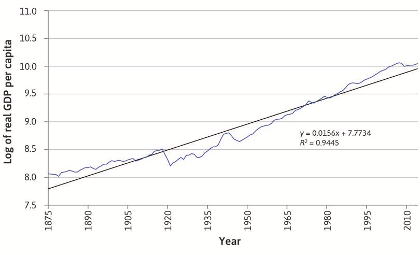
\includegraphics[width=\textwidth]{../QuestionBankImage/OUP-U13-Q04-01.png}

\begin{Exercise}




\Question (OUP-U17-Q4)
The figure shows that central banks reduced interest rates more sharply and kept them lower after the 2008 crisis than they did in the 1930s. But the figure shows nominal interest rates. Bearing in mind that inflation was slightly negative in the early 1930s and approximately zero from 2009, which of the following statements could be true about monetary policy after 1929 and after 2008?
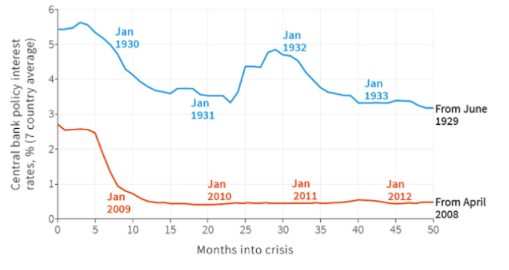
\includegraphics[width=\textwidth]{../QuestionBankImage/OUP-U17-Q4-01.png}
\answer{D}
\begin{tasks}(1)
    \task It is real (not nominal) rates that matter, so the figure tells us nothing useful.
        \details{The real interest rate is the nominal rate minus the rate of inflation. Given that you know inflation is negative in the early period and zero in the later period, you can use the figure to deduce approximate real interest rates and make some statements about monetary policy.}
    \task Since inflation is roughly zero, the nominal and real rates are the same in both periods.
        \details{This is correct for the later period, but what about the real rate in the earlier period?}
    \task When we account for inflation, there is little difference in the stance of monetary policy in the two periods.
        \details{Look again at the formula for the real interest rate. What is the real interest rate in the earlier period?}
    \task When we consider real interest rates, monetary policy was even tighter in the 1930s compared with 2008 onwards.
        \details{Given that prices were falling in the early 1930s, the real rate is even higher than the nominal rate shown in the figure. In the later period, with stable prices, the real and nominal rates are the same. So when we look at real rates, the gap between the two periods is even larger than it appears in the figure.}
\end{tasks}



\Question (OUP-U17-Q9)
In the diagram shown, demand for the industry’s goods falls from A to B. In the new equilibrium at C, individual firms are now receiving lower revenue. If they try to restore their earnings by producing more, which of the following is likely to happen in the short run?
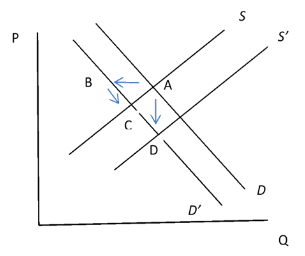
\includegraphics[width=\textwidth]{../QuestionBankImage/OUP-U17-Q9-01.png}
\answer{B}
\begin{tasks}(1)
    \task They will not be able to sell the additional output, so the market remains at C.
        \details{This assumes that the increase in supply has no effect on the equilibrium price and quantity, which seems unlikely.	The increase in supply will drive prices down even further (for example, to point D).}
    \task Producers face a catastrophic fall in prices, partly of their own making.
        \details{We can imagine a shift in the supply curve, assuming that in the short run firms are prepared to sell at prices that ignore costs of production. Doing so is unsustainable, and at point D many firms will go out of business. Supply will fall and prices will recover.}
    \task We cannot predict what will happen.
        \details{There may be some uncertainty regarding the exact quantity sold in the short run. However, provided the supply and demand schedules are based on firm evidence, we know that an increase in production must drive the price down further, with potentially catastrophic results. We can also make predictions based on similar events that happened in the past (in this case, the US farmers in the Great Depression).}
    \task The direction of price and quantity changes depends on the elasticity of demand.
        \details{It is quite correct that the actual size of the price and quantity movements depends upon the elasticity (or slope) of both the demand and supply curves. However, if the demand curve has a negative slope and the supply curve has a positive slope, we can be sure of the directions of adjustment.}
\end{tasks}




\Question (OUP-U17-Q11)
You are given the following information about the short-term nominal interest rate and the rate of inflation over a period of 8 years. In which year was the real rate of interest at its maximum and in which years might we regard monetary policy as having been expansionary?
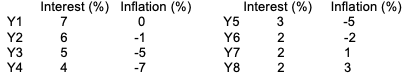
\includegraphics[width=\textwidth]{../QuestionBankImage/OUP-U17-Q11-01.png}
\answer{B}
\begin{tasks}(1)
    \task The real rate is at its maximum in Y4, but monetary policy is expansionary in all years since the rate of interest is falling.
        \details{The first part is correct. The real rate in Y4 is 11\% (= 4 - -7). However, the real rate has been rising since Y1 (7\%, 7\%, 10\%, 11\%) in spite of reductions in the nominal rate.	The real rate is at its maximum in Y4. It starts to fall in Y5 and falls below the Y1 rate in Y6.}
    \task Y6 is the earliest point at which we can describe monetary policy as expansionary.
        \details{The real rate is at its maximum in Y4. In spite of cuts to the nominal rate from Y1, the real rate does not fall below the rate in Y1 until we get to Y6 (= 4\%). The real rate does not turn negative until Y8.	The real rate is at its maximum in Y1 (= 7\%).}
    \task It only becomes negative in Y8, which is the earliest that we can describe policy as expansionary.
        \details{The real rate is higher in Y4 at 11\% (= 4 - -7). It is true that the real rate only becomes negative in Y8, but it falls below its initial (Y1) rate in Y6. We could argue that this reduction below the starting rate is where the expansionary policy starts.}
    \task The real rate is at its maximum in Y1 (=7\%) and monetary policy becomes expansionary in Y3 when the real rate falls to zero (= 5 - 5).
        \details{The real rate is at its maximum in Y4 at 11\% (= 4 - -7). In Y3, the real rate is actually 10\% (= 5 - -5). Note: we need to subtract a negative inflation rate.}
\end{tasks}



\Question (OUP-U17-Q20)
According to the original Phillips curve (Unit 15), higher inflation is associated with lower unemployment. The term ‘stagflation’ was coined to describe the unusual situation in the 1970s where unemployment and inflation both rose together. Which of the following best summarises the underlying causes?
\answer{D}
\begin{tasks}(1)
    \task Lower profits and a reduced rate of net investment meant a slower increase in productivity.
        \details{The Phillips curve says nothing about profits, investment, or productivity. These events may be involved in the change, but the answer does not explain how they contributed to high unemployment and inflation.}
    \task The lower growth of productivity meant a slower growth in the real wage and in the upward movement of the price-setting curve.
        \details{This may be correct, but does not explain the increase in unemployment.	The lower productivity growth of productivity meant slower real wage growth and a smaller upward movement of the price-setting curve. At the same time, the nature of industrial relations meant that the wage-setting curve also shifted upwards.}
    \task The result is that the wage and price-setting curves intersect at a lower employment (higher unemployment) rate than before.
        \details{This explains the higher levels of unemployment in the 1970s but not the higher rates of inflation that went with it.	The lower growth of productivity meant a slower growth in the real wage and in the upward movement of the price-setting curve. In addition, the succession of oil price shocks caused a rise in prices that firms could only partially pass on. This also ate into profits, reducing further the upward movement of the price-setting curve.}
    \task It also led people, workers especially, to expect inflation and therefore to build it into wage settlements.
        \details{This explains both the increase in unemployment and inflation.}
\end{tasks}



\Question (OUP-U17-Q22)
The leverage ratio is defined as total assets/equity. Assume that a household’s sole asset is a house worth \$190,000, which it has bought with a mortgage loan of \$180,000. What is the value of the leverage ratio, and what happens to the ratio if the house value falls to \$185,000?
\answer{A}
\begin{tasks}(1)
    \task 19; 37.
        \details{The ratio begins at 19 (= 190/10) and rises to 37 (185/5) as the value falls. Notice how the small change in the value dramatically changes the ratio.}
    \task 19; 18.5.
        \details{The ratio begins at 19 (= 190/10) and rises to 37 (185/5) as the value falls. Remember, the ratio divides the value of the asset by the value of equity. As the value falls, both the value and the equity fall.}
    \task 0.053; 0.027.
        \details{These are the inverse of the correct values. Remember, the leverage ratio divides the asset value by the equity value, not the other way round.}
    \task 19; 13.
        \details{19 is correct for the initial value but 13 is the value of the ratio if the price increases by \$5,000 (to \$195,000) instead of falling to \$185,000. Note again though how the small change in value has a large effect on the ratio.}
\end{tasks}



\Question (TEA-U17-Q1)
Herbert Hoover was the US President between 1929 and 1933. During this time: (1) President Hoover advocated a balanced budget which remained within the range of -0.6\% to +0.8\% of GNP in 1929-31, (2) Output was 20\% below the full employment level in 1931, (3) The short-term nominal interest rate fell from 5.8\% in 1929 to 1.7\% in 1933, (4) The CPI decreased from -2.7\% in 1930 to -10.3\% in 1932 and (5) The US remained on the gold standard while the UK abandoned the regime in 1931. hich of the following statements regarding this period is correct?
\answer{B}
\begin{tasks}(1)
    \task The government’s balanced budget contributed to the stabilisation of economic activity.
        \details{Given that the output was 20\% below the full employment level in 1931 there must have been a large decline in tax revenues. Therefore a balanced budget would have meant a large cyclically adjusted surplus. Thus in reality there was a large fiscal contraction.}
    \task Despite the cut in the nominal interest rate, monetary policy was contractionary during this period.
        \details{Even though the nominal interest rate fell, the real interest rate was rising because prices were falling.}
    \task The cut in the nominal interest rate was possible due to the US remaining in the gold standard.
        \details{Remaining in the gold standard meant that the nominal interest rate needed to be kept high relative to other countries in order to attract an inflow (or prevent the outflow) of gold. The nominal interest rate was cut to close to zero once the US left the gold standard in 1933.}
    \task The fact that the UK left the gold standard made it easier for the US to remain in the gold standard.
        \details{Once the UK left the gold standard there were expectations that the US would also leave, leading to a large outflow of gold. This made it difficult for the US to remain in the gold standard.}
\end{tasks}



\Question (OUP-U17-Q13)
Imagine that you are responsible for policymaking in an economy that is experiencing a deep recession. You and your colleagues announce a number of measures (like those in Roosevelt’s ‘New Deal’) that you tell everyone will boost demand and output. Why does it matter whether the public believes your announcement?
\answer{B}
\begin{tasks}(1)
    \task It does not. If the measures are appropriate, aggregate demand will increase, regardless of what anyone thinks.
        \details{Remember that lots of spending decisions have a forward-looking focus. This is especially true of firms’ investment plans but also of households’ decisions to buy durable goods. This immediately makes expectations relevant. If people believe that aggregate demand is going to increase (output rise, unemployment fall), they will feel more confident, spend more, and give a further boost to aggregate demand.}
    \task People will feel more confident about the future and increase their spending, which will reinforce the actions of government.
        \details{If people believe your announcement, they will feel more confident and may bring forward their spending plans or be encouraged to invest more. This helps to make your announcement something of a ‘self-fulfilling prophecy’. It is also similar to the positive feedback mechanism we discussed earlier in this unit.	If they really believe that you are going to increase government spending, they may worry that taxes will have to rise in future. They will reduce their spending in order to save more for the future tax demands, which will undermine your strategy.}
    \task It might be better if they simply ignored your promises.
        \details{It is always possible that people react adversely to policy announcements, especially if they do not understand them. This is why ‘presentation’ is often important and why Roosevelt stressed the need to be bold. In this case, to think that increasing public spending in a recession is a bad idea, people have to ignore the fact that such spending is likely to boost output, employment, and incomes, which is unlikely.}
    \task You are more likely to be re-elected if people believe that you tried to do something.
        \details{It is possible for policymakers to make these announcements and launch these plans in order to get re-elected. However, this is a dangerous strategy, because re-election is unlikely if these plans turned out to be a disaster. If people’s confidence in you as a policymaker matters, it must be because their confidence helps you bring about some improvement in the economy.}
\end{tasks}



\Question (OUP-U17-Q24)
It is well known that financial transactions frequently involve asymmetric information, because one party to the deal (usually the borrower) has better information about the risk and return to which the borrowed funds will be exposed than the other party (typically the lender). How does the concept of asymmetric information help us understand the particular events described in Section 17.11 (The role of banks in the crisis)?
\answer{C}
\begin{tasks}(1)
    \task Banks were reluctant to lend to households and firms because they did not know the risks involved.
        \details{This is not a special feature of the credit crunch. It is part of the general problem of asymmetric information and banks usually make credit assessments under conditions of normal uncertainty and ignorance. The problems referred to in the text concern the interbank market – the market through which banks lend to each other for very short periods – sometimes as short as overnight.}
    \task Central banks were reluctant to provide liquidity because they could not make an accurate assessment of which banks were solvent.
        \details{This was certainly a worry, but central banks reacted by relaxing their conditions, cutting the official interest rate, and trying to persuade banks to borrow. However, banks were reluctant to borrow from the central bank, probably because they feared that in the nervous atmosphere of the time, news that they had borrowed from the central bank would cause a panic amongst depositors.}
    \task In the credit crunch, banks were reluctant to lend to each other because they knew that risk was widespread because of large holdings of financial assets that were hard to value, and whose distribution amongst banks was unknown.
        \details{Banks knew the risk of default was generally high but could not pin down the risk for any individual bank. The probability of default could not be estimated and so the normal pricing formula (shown in the text) could not be used. This meant the safest strategy was not to lend at all. The interbank market seized up.}
    \task Households were reluctant to lend to banks because they could not assess their risk.
        \details{It is true that many households were nervous and wondered about withdrawing deposits. But bank deposits are money, and households need bank accounts to carry out everyday payments. Furthermore, the uncertainty about the future was causing many households to increase their savings and, in the first instance, this meant accumulating bank deposits.}
\end{tasks}



\Question (ECO-U17-Q3)
Franklin Roosevelt became the US President in 1933. In the period after he became the president: The federal government deficit increased to 5.6\% of GNP in 1934. The short-term nominal interest rate fell from 1.7\% in 1933 to 0.75\% in 1935. The CPI fell by 5.2\% in 1933 and rose by 3.5\% in 1934. The US left the gold standard in April 1933. The New Deal was launched in 1933 and included proposals to increase federal government spending in a wide range of programs and reforms to the banking system.  Which of the following statements is correct regarding the years immediately after Roosevelt became the US president?
\answer{A}
\begin{tasks}(1)
    \task A change in the expectations of consumers of their future earnings, as a result of the New Deal, would have contributed to an expansion in the economy’s aggregate demand.
        \details{More optimistic expectations lead to increased consumer spending, as shown in Figure 17.9.}
    \task The value of the US dollar increased as the result of the abandonment of the gold standard and allowed the nominal interest rate to be cut to close to zero.
        \details{The abandonment of the gold standard meant that the US dollar could be devalued, (from \$20.67 to \$35 per ounce of gold). It was no longer necessary to keep the interest rate high to maintain the dollar at the higher rate (meaning fewer dollars per ounce).}
    \task The real interest rate rose after 1933.
        \details{With the nominal interest rate falling, and with inflation turning positive from negative, the real interest rate fell sharply (and became negative in 1934).}
    \task Fiscal contraction from the increased government deficit would have contributed to the economy escaping from the Depression.
        \details{Increased government deficit means fiscal expansion.}
\end{tasks}




\Question (OUP-U17-Q21)
A household owns a house valued at \$190,000, which it has bought with a loan of \$180,000. It also has financial savings of \$10,000. Which of the following shows its net worth at the outset, the minimum amount the value of the house has to fall in order to put the household into negative equity (on the house), and the minimum amount the value of the house has to fall to make the household insolvent?
\answer{C}
\begin{tasks}(1)
    \task \$20,000; £20,000; \$20,001.
        \details{Net worth at the outset is \$20,000 (= \$10,000 financial assets + £10,000 home equity). However, a fall in house value of \$20,000 does more than create negative equity – it destroys the household’s net worth and puts on the verge of insolvency.}
    \task \$200,000; \$10,001; \$190,000.
        \details{\$200,000 is the household’s total wealth. Its net worth is total wealth minus debts = \$200,000 - \$180,000 = \$20,000. \$10,001 is sufficient to create negative equity since the value of the debt will be \$180,000 while the value of the house will be \$179,999. If the value of the house falls by \$190,000 it will be completely worthless and the household will certainly be insolvent. Its net worth will be financial assets (\$10,000) – debt (\$180,000) = -\$170,000. However, the test of insolvency is simply negative net worth (-\$1). This requires a fall in the value of the house of only \$20,001.}
    \task \$20,000; \$10,001; \$20,001.
        \details{Net worth at the outset is \$20,000 (= \$10,000 financial assets + £10,000 home equity). A fall in house value of \$10,001 wipes out the home equity. A fall of \$20,001 increases negative equity to £10,001, which is no longer covered by the value of financial assets.}
    \task \$200,000; \$10,001; \$20,001.
        \details{\$200,000 is the household’s total wealth. Its net worth is total wealth minus debts = \$200,000 - \$180,000 = \$20,000. The other two figures are correct.}
\end{tasks}

\end{Exercise}

\end{document}
